\section{Marco Teórico}
\subsection[Tecnologías]{Tecnologías: Lenguaje \& Librerias.}

\begin{frame}{Lenguaje de Programación}{Python}
    \begin{columns}
        \begin{column}{0.4\textwidth}
            % Aquí podrías incluir una imagen de ejemplo
            \centering
            \begin{figure}[H]
                \centering
                \adjustbox{max width=\textwidth, max height=0.5\textheight}{%
                
\includegraphics{img/marcoTeorico/python-logo.png}
                }
                \vspace{-0.25cm}
                \caption{\tiny~Logo de Python \textit{Adaptado de:}~\cite{PythonSoftwareFoundation}}%
                \label{fig:Python_logo}
            \end{figure}
        \end{column}
        \begin{column}{0.6\textwidth}
            \begin{itemize}
                \item Lenguaje de programación de alto nivel y propósito general
                \item Sintaxis clara y legible que favorece la productividad
                \item Multiparadigma: soporta programación orientada a objetos, imperativa y funcional
                \item Tipado dinámico y administración automática de memoria
                \item Extensa biblioteca estándar
            \end{itemize}
        \end{column}
    \end{columns}
\end{frame}

\begin{frame}{Biblioteca de Simulación N-Cuerpos}{REBOUND}
    \begin{columns}
        \begin{column}{0.6\textwidth}
            \begin{itemize}
                \item Implementado en C con interfaz Python muy completa
                \item Enfocado en dinámica colisional y no colisional, N-cuerpos de propósito general
                \item Integradores avanzados: Leapfrog, Wisdom-Holman (WHFast), SEI (Simpléctico Epicíclico), IAS15
                \item Algoritmos de gravedad: Suma directa, Barnes-Hut (Octree)
                \item Detección y resolución de colisiones físicas
            \end{itemize}
        \end{column}
        \begin{column}{0.4\textwidth}
            % Aquí podrías incluir una imagen de ejemplo
            \centering
            \begin{figure}[H]
                \centering
                \adjustbox{max width=1.4\textwidth, max height=0.5\textheight}{%
                
\includegraphics{img/marcoTeorico/reboundblack-logo.png}
                }
                \vspace{-0.25cm}
                \caption{\tiny~Logo de REBOUND \textit{Adaptado de:}~\cite{Rein2012}}%
                \label{fig:REBOUND_logo}
            \end{figure}
        \end{column}
    \end{columns}
\end{frame}

\begin{frame}{Biblioteca de Optimización}{pymoo}
    \begin{columns}
        \begin{column}{0.4\textwidth}
            % Aquí podrías incluir una imagen de ejemplo
            \centering
            \begin{figure}[H]
                \centering
                \adjustbox{max width=\textwidth, max height=0.5\textheight}{%
                
\includegraphics{img/marcoTeorico/pymoo-logo.png}
                }
                \vspace{-0.25cm}
                \caption{\tiny~Logo de pymoo \textit{Adaptado de:}~\cite{blank2020}}%
                \label{fig:pymoo_logo}
            \end{figure}
        \end{column}
        \begin{column}{0.6\textwidth}
            \begin{itemize}
                \small
                \item Framework moderno para optimización multiobjetivo (y mono-objetivo)
                \item Amplia gama de algoritmos: NSGA-II, NSGA-III, MOEA/D, RVEA, CMA-ES, DE, GA, PSO
                \item Alta flexibilidad para definir problemas, operadores y algoritmos personalizados
                \item Excelente para análisis multiobjetivo con herramientas específicas
                \item Soporte para paralelización (Dask, multiprocessing)
            \end{itemize}
        \end{column}
    \end{columns}
\end{frame}

\begin{frame}{Biblioteca de Visualización}{Matplotlib}
    \begin{columns}
        \begin{column}{0.6\textwidth}
            \begin{itemize}
                \item Biblioteca estándar para visualización en Python
                \item Gran flexibilidad y personalización
                \item Excelente para gráficos científicos
                \item Amplia documentación y comunidad
            \end{itemize}
        \end{column}
        \begin{column}{0.4\textwidth}
            % Aquí podrías incluir una imagen de ejemplo
            \centering
            \begin{figure}[H]
                \centering
                \adjustbox{max width=\textwidth, max height=0.5\textheight}{%
                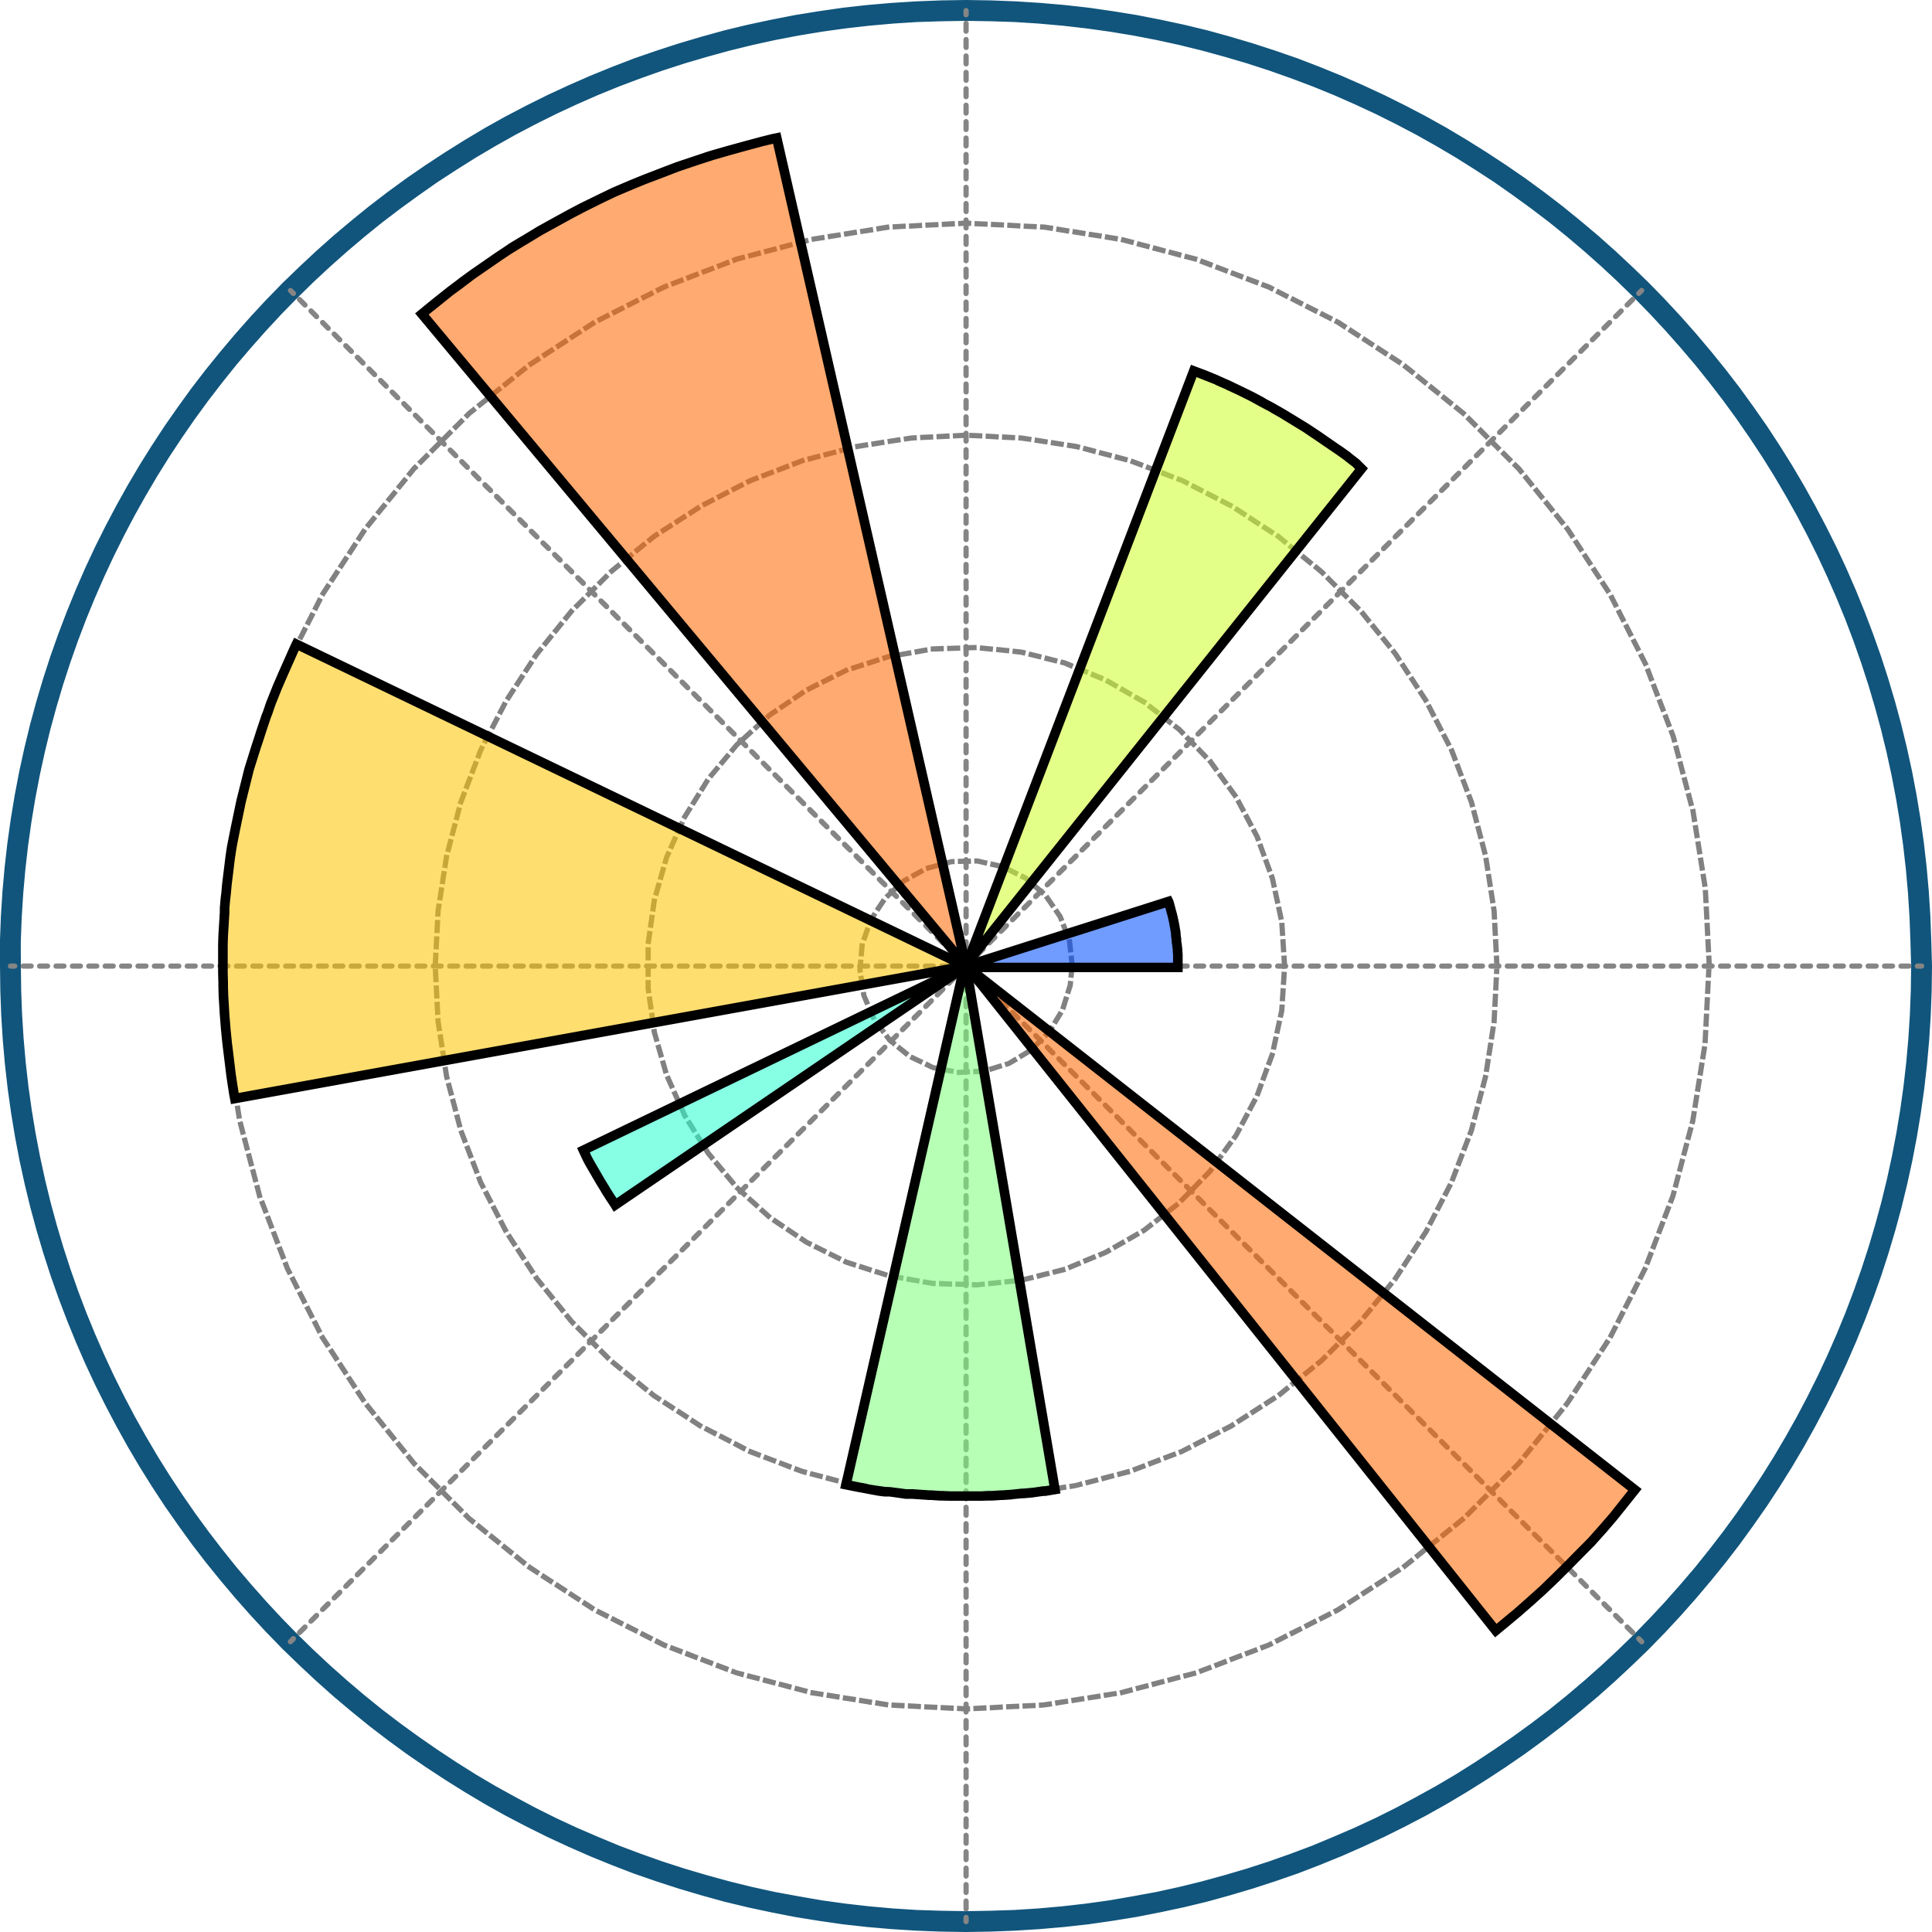
\includegraphics{img/marcoTeorico/matplotlib-logo.png}
                }
                \vspace{-0.25cm}
                \caption{\tiny~Logo de Matplotlib \textit{Adaptado de:}~\cite{Hunter:2007}}%
                \label{fig:Matplotlib_logo}
            \end{figure}
        \end{column}
    \end{columns}
\end{frame}

\begin{frame}{Biblioteca de GUI para Python}{PyQt}
    \begin{columns}
        \begin{column}{0.4\textwidth}
            % Aquí podrías incluir una imagen de ejemplo
            \centering
            \begin{figure}[H]
                \centering
                \adjustbox{max width=\textwidth, max height=0.5\textheight}{%
                
\includegraphics{img/marcoTeorico/qt-logo.png}
                }
                \vspace{-0.25cm}
                \caption{\tiny~Logo de PyQt.~\textit{Adaptado de:}~\cite{qt_wiki}}%
                \label{fig:PyQt_logo}
            \end{figure}
        \end{column}
        \begin{column}{0.6\textwidth}
            \begin{itemize}
                \item Basado en Qt (C++), con aspecto profesional y moderno
                \item Extensa colección de widgets y sistema potente de layouts
                \item Excelente integración con Matplotlib y otras librerías gráficas
                \item Buen soporte para multihilo con señales y slots
                \item Qt Designer para diseño visual de interfaces
            \end{itemize}
        \end{column}
    \end{columns}
\end{frame}

\subsection[Métodos \& Técnicas]{Métodos \& Técnicas a utilizar.}

\begin{frame}{Cálculo de Gravedad y Colisiones}{Mediante módulos de \texttt{REBOUND}}
    \begin{columns}
        \begin{column}{0.6\textwidth}
            \small
            \begin{itemize}
                \item \textbf{Cálculo de Gravedad:}
                \begin{itemize}
                    \item \textbf{Suma Directa:} $O(N \cdot N_{\text{active}})$, exacta, ideal para pocos cuerpos
                    \item \textbf{Octree (Barnes-Hut):} $O(N \log N)$, aproximada, eficiente para $N > 10^2$
                \end{itemize}
                \item \textbf{Detección de Colisiones:}
                \begin{itemize}
                    \item \textbf{Búsqueda Directa:} $O(N^2)$, exacta para esferas duras
                    \item \textbf{Octree:} $O(N \log N)$, para geometrías 3D generales
                    \item \textbf{Barrido Plano:} Eficiente para geometrías cuasi-2D
                \end{itemize}
            \end{itemize}
        \end{column}
        \begin{column}{0.4\textwidth}
            % Aquí podrías incluir una imagen de ejemplo
            \centering
            \begin{figure}[H]
                \centering
                \adjustbox{max width=\textwidth, max height=0.5\textheight}{%
                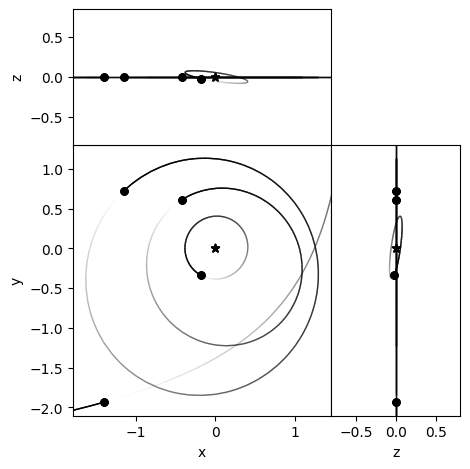
\includegraphics{img/marcoTeorico/rebound-simulation.png}
                }
                \vspace{-0.25cm}
                \caption{\tiny~Simulación de orbitas usando REBOUND \textit{Adaptado de:}~\cite{rebound_hyperbolic_orbits_2025}}%
                \label{fig:REBOUND_methods}
            \end{figure}
        \end{column}
    \end{columns}
\end{frame}

\begin{frame}{Enfoque del Proyecto}{Factibilidad y Optimización}
    \begin{columns}
        \begin{column}{0.4\textwidth}
            % Aquí podrías incluir una imagen de ejemplo
            \centering
            \begin{figure}[H]
                \centering
                \adjustbox{max width=\textwidth, max height=0.5\textheight}{%
                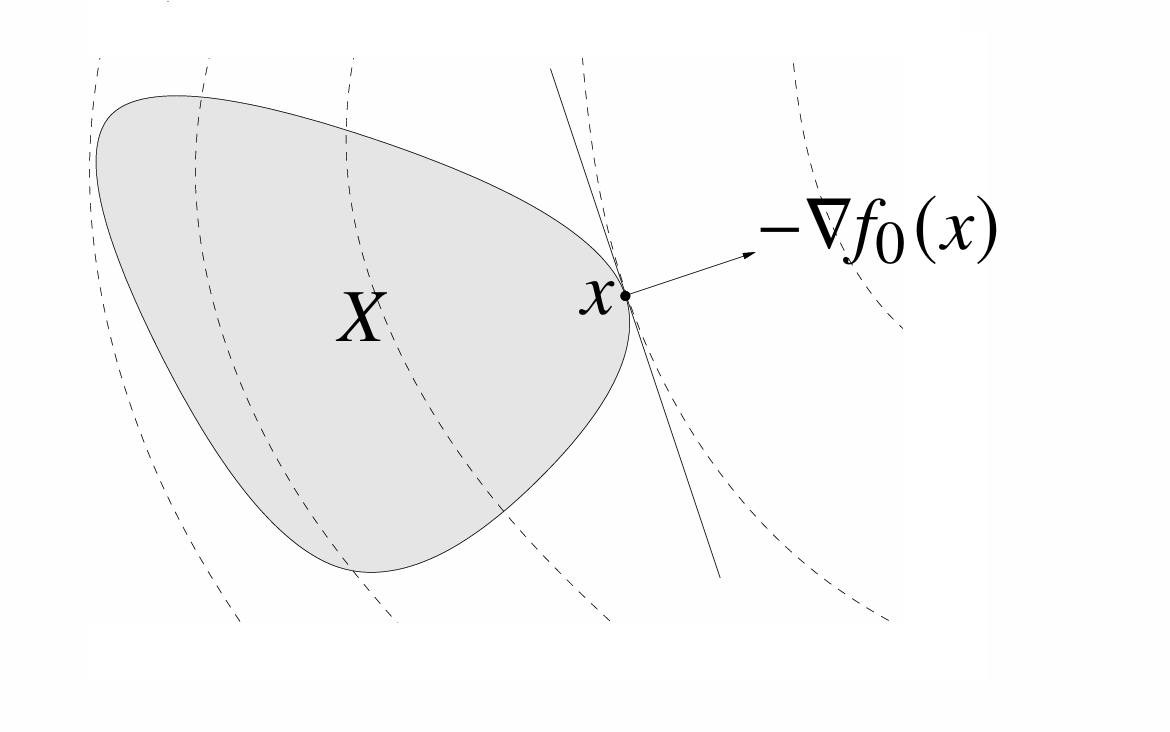
\includegraphics{img/marcoTeorico/optimizacion_fig1.png}
                }
                \vspace{-0.25cm}
                \caption{\tiny~Gráfica 2D que muestre contornos de una función objetivo $f_0(x)$,
                        una región factible sombreada definida por restricciones, y el punto óptimo $x^*$.\ \textit{Adaptado de:}~\cite{BoydVandenbergheSlides2023}}%
                \label{fig:factibility_optimization}
            \end{figure}
        \end{column}
        \begin{column}{0.6\textwidth}
            \small
            \begin{itemize}
                \item \textbf{Problema de Factibilidad (Núcleo):}
                \begin{itemize}
                    \item Determinar si existen configuraciones estables
                    \item Criterio clave: Exponente de Lyapunov $\lambda_1 \leq \text{umbral}$
                    \item Restricciones físicas. %masas positivas, parámetros orbitales válidos
                \end{itemize}
                \item \textbf{Marco de Optimización:} % (Herramienta)
                \begin{itemize}
                    \item Función objetivo: minimizar $\lambda_1$ directamente
                    \item Algoritmo Genético como herramienta exploratoria
                    \item Permite búsqueda eficiente en el espacio de parámetros
                \end{itemize}
            \end{itemize}
        \end{column}
    \end{columns}
\end{frame}

\begin{frame}{Algoritmo de Exploración}{Algoritmo Genético (AG) con pymoo}
    \begin{columns}
        \begin{column}{0.6\textwidth}
            \small
            \begin{itemize}
                \item \textbf{Componentes principales:}
                \begin{itemize}
                    \item \textbf{Muestreo:} FloatRandomSampling() para población inicial %chktex 36
                    \item \textbf{Selección de Padres:} TournamentSelection
                    \item \textbf{Cruce:} SBX (Simulated Binary Crossover)
                    \item \textbf{Mutación:} PolynomialMutation para variables continuas
                    \item \textbf{Manejo de Restricciones:} out[``G''] para restricciones físicas
                \end{itemize}
                \item \textbf{Parámetros clave:} Tamaño de población, eliminación de duplicados, semilla aleatoria para reproducibilidad
            \end{itemize}
        \end{column}
        \begin{column}{0.4\textwidth}
            % Aquí podrías incluir una imagen de ejemplo
            \centering
            \begin{figure}[H]
                \centering
                \adjustbox{max width=\textwidth, max height=0.5\textheight}{%
                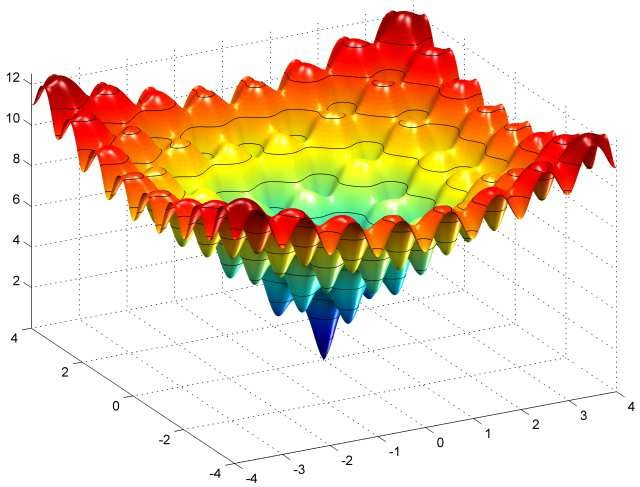
\includegraphics{img/marcoTeorico/benchmarkfunction.png}
                }
                \vspace{-0.25cm}
                \caption{\tiny~Funcion tipo benchmark, para la evaluación de AGs \textit{Adaptado de:}~\cite{silva2018}}%
                \label{fig:genetic_algorithm}
            \end{figure}
        \end{column}
    \end{columns}
\end{frame}

\begin{frame}{Indicador de Estabilidad}{Exponente de Lyapunov}
    \begin{columns}
        \begin{column}{0.4\textwidth}
            % Aquí podrías incluir una imagen de ejemplo
            \centering
            \begin{figure}[H]
                \centering
                \adjustbox{max width=\textwidth, max height=0.5\textheight}{%
                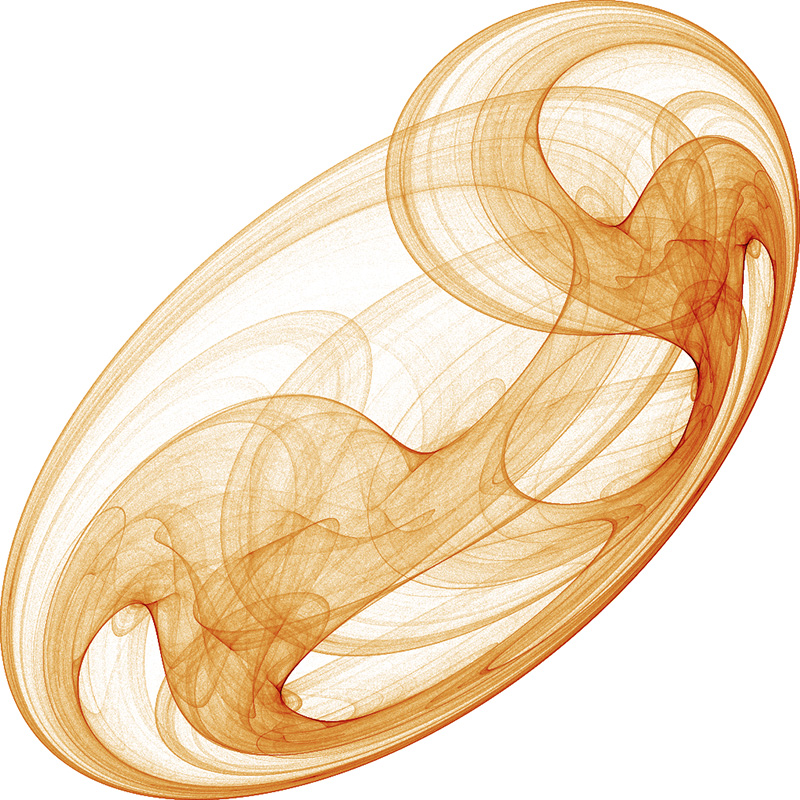
\includegraphics{img/marcoTeorico/lyapunovExponent-in-randomAttractors.jpg}
                }
                \vspace{-0.25cm}
                \caption{\tiny~Atractor caótico generado mediante exponentes de Lyapunov.~\textit{Adaptado de:}~\cite{bourke_lyapunov_attractors_2001}}%
                \label{fig:Lyapunov_diagram}
            \end{figure}
        \end{column}
        \begin{column}{0.6\textwidth}
            \begin{itemize}
                \item Cuantifica la sensibilidad a condiciones iniciales
                \item Indicador primario de estabilidad/caos: $\lambda_1 > 0$ implica comportamiento caótico
                \item Medida objetiva y cuantitativa de la estabilidad dinámica
                \item Permite predecir comportamiento a largo plazo
                \item Base matemática rigurosa (Teorema de Oseledec)
            \end{itemize}
        \end{column}
    \end{columns}
\end{frame}

